% Use only LaTeX2e, calling the article.cls class and 12-point type.

\documentclass[12pt]{article}

% Users of the {thebibliography} environment or BibTeX should use the
% scicite.sty package, downloadable from *Science* at
% www.sciencemag.org/about/authors/prep/TeX_help/ .
% This package should properly format in-text
% reference calls and reference-list numbers.



\usepackage[pdftex]{graphicx}

\usepackage[labelfont=bf]{caption}

\usepackage{indentfirst}

\usepackage{scicite}

% Use times if you have the font installed; otherwise, comment out the
% following line.

\usepackage{times}

% The preamble here sets up a lot of new/revised commands and
% environments.  It's annoying, but please do *not* try to strip these
% out into a separate .sty file (which could lead to the loss of some
% information when we convert the file to other formats).  Instead, keep
% them in the preamble of your main LaTeX source file.


% The following parameters seem to provide a reasonable page setup.

\topmargin 0.0cm
\oddsidemargin 0.2cm
\textwidth 16cm 
\textheight 21cm
\footskip 1.0cm


%The next command sets up an environment for the abstract to your paper.

\newenvironment{sciabstract}{%
\begin{quote} \bf}
{\end{quote}}


% Include your paper's title here

\title{Critical brain: the statistical physics of neural systems} 


% Place the author information here.  Please hand-code the contact
% information and notecalls; do *not* use \footnote commands.  Let the
% author contact information appear immediately below the author names
% as shown.  We would also prefer that you don't change the type-size
% settings shown here.

\author
{Kevin Gilmore}

%%%%%%%%%%%%%%%%% END OF PREAMBLE %%%%%%%%%%%%%%%%



\begin{document} 

% Double-space the manuscript.

\baselineskip24pt

% Make the title.

\maketitle 



% Place your abstract within the special {sciabstract} environment.

\begin{sciabstract}

\end{sciabstract}


\section*{Introduction}

The human brain is amazingly complex. Comprised of tens of billions of neurons with a hundred trillion connecting synapses, it's no wonder it remains so poorly understood. From this immensely complex network of interacting elements arise collective dynamics, which neuroscience research has only recently turned its focus to. However, the study of collective phenomena is well known to physics. Statistical mechanics uses probability theory to ascertain the collective behavior of systems made up of very large numbers of constituents, thereby connecting the microscopic to the macroscopic. The field of statistical mechanics has had great success in explaining not only the microscopic basis of thermodynamics, but also the emergence of macroscopic dynamics in complex systems outside the typical purview of physics. With this interdisciplinary mindset, some theorized the brain could operate in a regime characterized by statistical mechanics as a continuous phase transition\cite{Bak1987a}. Little credence was given to such theories until the publication of the first experimental evidence that neuronal networks exhibit avalanches reminiscent of a system operating at criticality \cite{Beggs2003b}.

In this paper I will discuss recent work in the emerging subfield of criticality in neural systems. Work in this field combines experimental neuroscience, nonlinear dynamics, complex systems, and graph theory in the context of statistical physics. To understand the human brain, and thus our behavior and cognition, necessitates the elucidation of the patterns of spatiotemporal brain activity that arise out of collective neural dynamics. To this end, the tools of statistical mechanics, and in particular those dealing with critical phenomena, may be of great use.

\paragraph*{Motivation}

Understanding the underlying mechanism by which the brain adaptively produces a broad range of behaviors is a fundamental problem in neuroscience. Indeed, the mechanism responsible for the emergence of behavior from simple excitable elements (neurons) interacting via electrochemical impulses is of ultimate importance in understanding intelligent life. Naturally, a subject of such fundamental interest and great complexity, but which can nonetheless be modeled simply, attracts physicists. 

Of course, mere interest does not suffice. Does physics really have something to contribute to the field of neuroscience in the context of neuronal networks? In the course of this paper, I will argue yes it does. The facts that networks of excitable elements operating at criticality benefit from maximal dynamic range \cite{Kinouchi2006b,Shew2009b} and information capacity\cite{Shew2011a} show that a statistical mechanical approach to understanding neuronal networks, and thus the brain, has real functional yield.

\section*{Physics of Phase Transitions and Critical Phenomena}

Statistical physics has had great success in explaining the emergence of macroscopic thermodynamic behavior from the underlying microscopic, atomic interactions. An emergent phenomena is a macroscopic one that can be explained simply, though it arises out of complicated microscopic interactions. Many interdisciplinary fields have attempted to make use of statistical mechanics to explain phenomena arising out of complicated dynamics. Continuous phase transitions are interesting because they exhibit a qualitative change in macroscopic behavior as a certain physical property continuously changes. A physical property that undergoes such a change and allows for distinguishing distinct phases is known as an order parameter. The critical point in a continuous phase transition is the point at which certain physical properties of the system in question are singular and the system itself is in some sense teetering between two phases, between two qualitatively different states such as order and disorder. For example, as its temperature is increased a magnet may undergo a second order phase transition from ferromagnet to paramagnetic. As the system approaches a critical temperature, known as the Curie temperature, the magnetization vanishes continuously. At the critical temperature, the magnetization fluctuates wildly corresponding to neither an ordered ferromagnetic nor disordered paramagnetic state. Two main features of continuous phase transitions are scale-invariance and universality. That a phase transition is scale-invariant means fluctuations occur at all length scales, and so such systems are statistically invariant under changes in length scale. Universality signifies a lack of dependence on microscopic properties near the critical point. As a result, widely different microscopic systems can display the same macroscopic behavior at a phase transition. The same scale-invariant theory can be used to describe many different systems. Properties such as susceptibility, specific heat, and correlation lengths have power law singularities at the critical point. The critical exponents corresponding to these power laws  may be shared between seemingly disparate systems such as ferromagnets and liquid-gas systems, which as a result may both be modeled by the Ising model. The Ising model is a mathematical model consisting of interacting spins on lattice. This spins take values of +1 or -1 and are coupled together through an interaction strength parameter. The 2D Ising model is one of the simplest models demonstrating a phase transition, illustrated in Figure 1. \cite{Sethna2011a}

\begin{figure}      
  \begin{center}    
 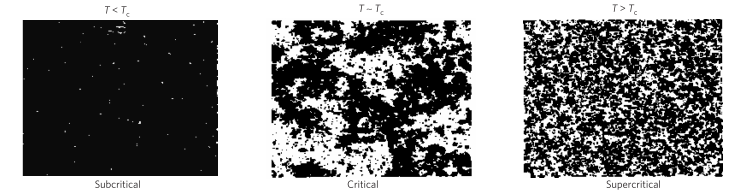
\includegraphics[width=1.1\textwidth]{Isingchialvo}    
    \caption{\textbf{2D Ising model.} Snapshots of spin configurations demonstrating a continuous phase transition. White pixels correspond to spin up (+1), while black is spin down (-1). In the subcritical and supercritical states homogenous order and disorder reign, respectively. At the critical temperature fluctuations occur on all length scales due to highly correlated sections. \cite{Chialvo2010a}}   
   \label{Figure::Ising model criticality}   
  \end{center}     
   \end{figure}
   


\paragraph*{Critical phenomena applied}

A number of physical systems are characterized by a wide range of event sizes that often are triggered in impulsive avalanches of activity, where the number of avalanches of a given size follows a power law $ D(s) \sim s^{-\tau} $ over several orders of magnitude. At criticality, these avalanches span the size of the system. This power law behavior results in a distinctive probability distribution in size. Such systems may be studied as critical points with the same tools as those in the study of continuous phase transitions. Earthquakes are an example of one such phenomena\cite{Sethna2011a}. An earthquake is caused by the grinding of two sides of a fault in a stick-slip type motion. The faults remain stuck for small applied stresses, and with strong stresses the faults simply slide by each other. However, at the transition between these two qualitatively different behaviors is a critical regime where earthquakes of all sizes are seen.  

\begin{figure}      
  \begin{center}    
 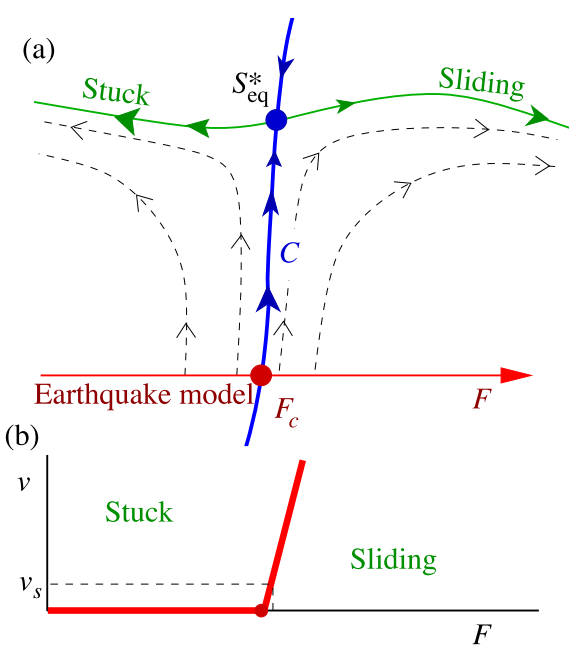
\includegraphics[width=.30\textwidth]{sethnaRGquakes}    
    \caption{\textbf{Model of self-organized criticality in earthquakes.} (a) The phases of stuck faults and sliding faults are separated by a critical manifold C. The transition between phases is caused by an external stress F. Along C fluctuations allow for earthquakes of all sizes. (b) Velocity vs force plot for stuck-sliding transition. Continental drift drives the fault at a constant velocity and sets the force to $F_{c}$. \cite{Sethna2011a}}   
   \label{Figure::Power law behavior in earthquakes}   
  \end{center}     
   \end{figure}

\paragraph{Self-organized criticality} 

The critical point in a system typically may only be reached by fine tuning the system's parameters. An interesting exception to this is a dynamical system whose critical point acts as an attractor. In such a system, no fine tuning is necessary and despite starting far from equilibrium the critical regime may be reached. Bak's sandpile model\cite{Bak1987a} was the first example of a dynamical system displaying such self-organized criticality. Grains of sand are gradually and randomly added to a pile. As the pile of sand grows, if the slope becomes too large the pile will collapse via avalanche. The cycle of growth and collapse continues until the slope reaches a point wherein the pile is barely stable to small perturbations. Dropping another grain of sand may trigger a catastrophic avalanche, or perhaps nothing at all. That is, there is no characteristic length scale at this point. Apparently this system is attracted to its critical point with no tuning of a system parameter - unlike more typical examples of critical phenomena. The sandpile model demonstrates avalanches that follow power law behavior for both the distribution of event sizes and durations over many orders of magnitude, and it does so without the fine tuning of any particular parameter. Such a system is said to exhibit self-organized criticality. It turns out the previously described earthquake model also is self-organized: a small velocity applied by continental drift naturally sets the appropriate external force to drive critical fluctuations\cite{Sethna2011a}. Figure 2 illustrates this model. 


\section*{Networks and Graph Theory}

Networks, individuals and the complicated interconnections between them, are described mathematically by graphs. In graph theory, the network's topology is represented as a collection of nodes with links that connect them. An adjacency matrix is used to represent a graph in more explicit mathematical form. Each row and column represents a node, and the elements of the matrix correspond to either 1 for a link or 0 for no link between the ith and jth node.

Branching processes were originally studied in the context of the survival of aristocratic family names in the Victorian era. Galton and Watson modeled the passing on of family names with an active (or excited) node branching to other nodes (father to sons) which in turn are active with some probability \cite{Watson2014}. The threshold for the longevity of a family name is met when the average number of active nodes from generation to generation is unchanged. Should the average number of active nodes increase (decrease), the process is dubbed supercritical (subcritical). In the subcritical case the family name dies out. Figure 3 illustrates branching processes in these three regimes. More recently, such branching processes have been used to model the propagation of disease, for example. The propagation of excitations in a branching process behaves as the avalanches previously described. In the case of a critical branching process, the sum of the probabilities of the nodes excited from one generation to the next is equal to one. This sum is known as the branching ratio. In this regime, both the size (s) and duration (t) of the avalanches follow power laws $ D(s) \sim s^{-3/2} $ and $ D(t) \sim t^{-2} $, respectively. \cite{Larremore2014}

\begin{figure}      
  \begin{center}    
 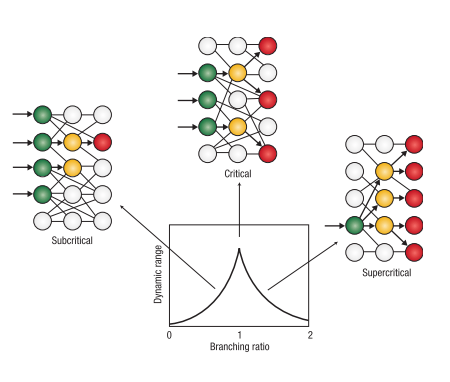
\includegraphics[width=.7\textwidth]{Branchingprocesschialvo}    
    \caption{\textbf{Branching processes.} Subcritical branching processes quickly die out, while the system is saturated in the supercritical regime. Only in the critical state with $\sigma = 1$ is the input activity maintained, on average. At criticality, the system is sensitive to both small and large pertubations, thus maximizing its dynamic range. \cite{Chialvo2006a}}   
   \label{Figure::Critical Branching Process}   
  \end{center}     
   \end{figure}

\section*{Experiments in Neuroscience}

The brain is composed of networks of tens of billions of neurons. The large number of interacting elements - neurons - qualifies the brain as a complex system. In general, such complex systems are characterized by a noisy, chaotic state with very weak interactions and a frozen, static state with very strong interactions - with a mediating critical junction. Given that the brain must maintain some order to ensure consistent behavioral responses to particular stimuli as well as some degree of disorder to enable flexibility in the form of adaptive changes to a dynamic environment, it was speculated in the 90s that the brain could be operating at criticality \cite{Bak1987a}. Of course, typically the critical regime a complex system passes through during a continuous phase transition is only accessible via fine tuning of system parameters. This was appropriately  thought to be unrealistic in the brain. However, the concepts of self-organized criticality re-opened the door for the study of criticality in the brain.

Motivated by the work done in modeling complex systems such as earthquakes and forest fires as networks at criticality, neuroscientists began looking for experimental evidence that similar processes could be happening in networks of neurons. To determine if this is the case, neuronal avalanches described by power laws would have to be seen. In 2003, the first experimental evidence that neuronal activity does involve neuronal avalanches - impulsive propagation of activity from individual neurons firing and triggering subsequent neurons to fire - was published\cite{Beggs2003b}. By studying the propagation of spontaneous neuronal activity in slices of rat cortex on multielectrode arrays, Beggs and Plenz observed avalanches of signal with size distribution $ D(s) \sim s^{-3/2} $.  This data is reproduced in Figure 4. Avalanches occur up to the size of the system (the number of electrodes), which is consistent with avalanches occurring at a critical point. Over 2 orders of magnitude the distribution is a power law with exponent -3/2. In addition, the branching parameter, i.e. the number of neurons excited step-by-step during the avalanche, is about 1. These neuronal avalanches do follow power laws just as would be expected from a critical branching process. See Figure 5 for comparison of neuronal avalanches in several systems, from cultured slices of cortex to awake humans. 
 
\begin{figure}      
  \begin{center}    
 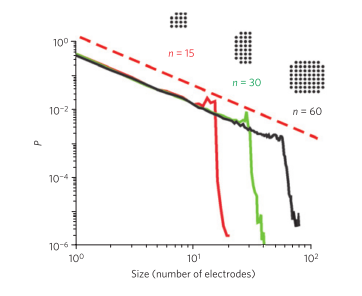
\includegraphics[width=.6\textwidth]{originalavalancheplenz}    
    \caption{\textbf{Size distribution of neuronal avalanches} in cortical cultured networks follows a power law with exponent of approximately -3/2 (dashed line). Insets indicate number of electrodes, and thus network size. Avalanches occur up to system size. \cite{Beggs2003b}} 
   \label{Figure::Neuronal Avalanches}   
  \end{center}     
   \end{figure}
   
\begin{figure}      
  \begin{center}    
 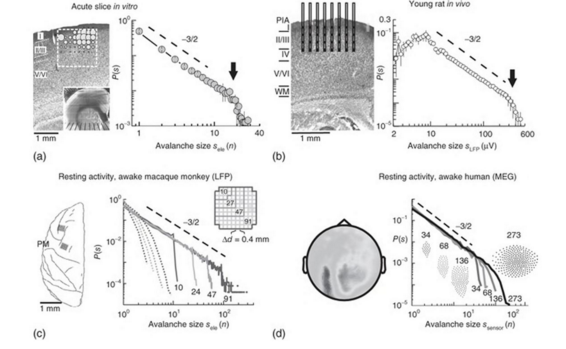
\includegraphics[width=.9\textwidth]{avalanchesplenzbook}    
    \caption{\textbf{Comparison of neuronal avalanches in several systems.} (a) Neuronal avalanches in cortex slice \textit{in vitro}. (b) Neuronal avalanches in rat \textit{in vivo}. (c) Neuronal avalanches in awake macaque monkey. Cutoff corresponds to area of array i.e. number of electrodes. (d) Neuronal avalanches in the resting MEG of he human brain. Sensor array size noted in inset and by grayscale and numbers on plot. \cite{Plenz2014}}
   \label{Figure::Neuronal avalanches in vitro and in vivo}   
  \end{center}     
   \end{figure}

Experimental evidence points towards networks of neurons operating in a critical regime characterized by power laws, but simply observing a trend in data that follows a power law does not establish the presence of critical phenomena. Some physical parameters must be shown to pass through a singularity, and the generative mechanism of the phenomena should be theoretically described. In addition, the use of the concept of criticality ought to be applied only if it yields some insight. Crucially, if the critical brain story is to be legitimized there must be a reason, a functional purpose for this supposed phenomena.   
      
\section*{Putting it all together}

The brain is an information processor. Over millennia it has evolved to its current state as one of the most complicated and poorly understood systems known. Any theory purported to describe neuronal networks should account for what we know about the information processing capabilities of the brain. Here is where the theory of criticality in networks provides something novel. Through both theoretical models and experimental findings, it has been shown that networks of neurons (indeed, any kind of complex network comprised of similar elements) achieve maximal information capacity and dynamic range at criticality. The significance of these findings is that there is a functional benefit to maintaining a critical state in the brain.

\begin{figure}      
  \begin{center}    
 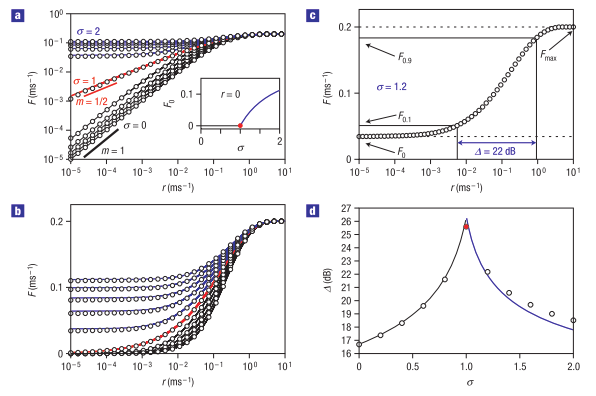
\includegraphics[width=.8\textwidth]{dynamicrangetheorycopelli}    
    \caption{\textbf{Response curves and dynamic range.} \textbf{(a)} Average activity F versus stimulus rate r with branching parameters from $\sigma = 0$ to 2 in intervals of .2. Represented as a log-log plot. \textbf{(b)} Lin-log plot of \textbf{(a)}. \textbf{(c)} Response curve for $\sigma = 1.2$ with dynamic range $\Delta$ from $10\%$ to $90\%$ of saturated response. \textbf{(d)} Dynamic range versus branching ratio. Optimization occurs at the critical point $\sigma = 1$.\cite{Kinouchi2006b}}   
   \label{Figure::Dynamic Range Theory}   
  \end{center}     
   \end{figure}
   
\paragraph{Theory}
The intensity of human-detectable physical stimuli, such as light and sound, varies by several orders of magnitude. For hearing the dynamic range is on the order of 140dB, for sight it's 90dB. This very large dynamic range must be accounted for in the model. Since single neurons respond in a linear, saturating way with a limited range, the broad dynamic range must be a collective phenomena. Kinouchi and Copelli found that a network of excitable elements, such as a neuronal network, has its dynamic range and sensitivity maximized at its critical point during a non-equilibrium phase transition\cite{Kinouchi2006b}. This is consistent with and lends further credence to the brain operating at criticality. Figure 6 shows the results of the simulations. The dynamic range is calculated from the $10\%-90\%$ response interval and is seen to be maximized at the critical branching ratio. In the subcritical regime, the dynamic range increases with the branching ratio. In the supercritical regime, the dynamic range decreases with the branching ratio. \cite{Larremore2011a, Larremore2012a}

\paragraph{Experiment}
The ability of a neuronal network to process information is determined by the neural activity it produces. Activity patterns in cortex cultures, anesthetized rats, and awake monkeys were measured to quantify their dynamic range (Figure 7) and information capacity (Figure 8). Experiment has demonstrated that networks generating neuronal avalanches benefit from maximized dynamic range\cite{Shew2009b}. By measuring the responses to a range of stimuli amplitudes, the dynamic range was computed by way of the same response interval as in the theoretical approach.

\begin{figure}      
  \begin{center}    
 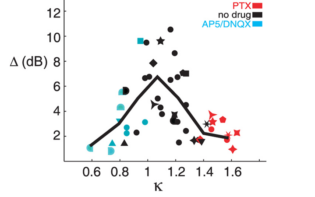
\includegraphics[width=.5\textwidth]{dynamicrangeexpplenz}    
    \caption{\textbf{Dynamic range.} Experimental data taken with no administered drug (black) a drug that reduces inhibition (red) and a drug that reduces excitation (blue). Dynamic range peaks near $\kappa = 1$. $\kappa$ is a measure of the difference between experimental results and theoretical reference and is nearly linearly related to the branching parameter $\sigma$. $\kappa \cong 1$ corresponds to the critical regime where $\sigma = 1$. \cite{Shew2009b}}   
   \label{Figure::Dynamic Range Experiment}   
  \end{center}     
   \end{figure}
  
\begin{figure}      
  \begin{center}    
 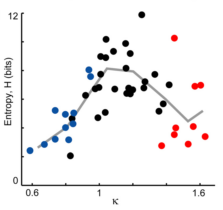
\includegraphics[width=.40\textwidth]{entropyplenz}    
    \caption{\textbf{Information capacity.} Experimental data taken with same drug-color scheme as previous figure. Information entropy is maximized around $\kappa = 1$. \cite{Shew2011a}}   
   \label{Figure::Entropy / information maximized experimental}   
  \end{center}     
   \end{figure}
   
In a similar study, it was found that in changing the ratio of excitation to inhibition in these subjects by way of excitory and inhibitory drugs, information capacity is maximized at a balanced ratio corresponding to the emergence of neuronal avalanches \cite{Shew2011a}. Multielectrode arrays comprised of an 8x8 grid of electrodes were used to record events, with 1 bit assigned to each electrode. Thus different activity levels correspond to distinct binary patterns. Shannon entropy, defined as

\begin{equation}
H = - \sum^{n}_{i=1}p_{i}\log_{2}p_{i},
\end{equation}

\noindent where n is the number of binary patterns and $ p_{i} $ is the probability that a particular pattern $i$ occurs, was calculated to quantify the information capacity. The agreement between experimental findings and theoretical models supports the theory of neuronal networks operating at criticality and suggests that in networks with balanced excitation and inhibition maximal information processing capabilities arise as a result of criticality. 

To summarize these experimental and theoretical findings, neuronal avalanches with power law distributions in size and duration were observed and found to maximize neuronal information processing in the form of dynamic range and information capacity (information entropy). These findings are consistent with the theory that neuronal networks operate at criticality. 

\paragraph{The Ising Model}
Additional work has been done in the field in an attempt to further bridge the gap between statistical physics and neuroscience. In particular, analogies have been drawn between Ising model dynamics and brain dynamics \cite{Fraiman2009a}. By transforming brain fMRI data and a 2D Ising model simulation into correlation networks, the two may be appropriately compared. A correlation network is here defined by linking sites with the strongest correlations. Correlations between lattice sites in the Ising model as well as sites from recorded brain data are computed, with links between sites defined whenever the correlation is greater than or equal to a given threshold. By setting this threshold, the average degree of the network may be regulated. The degree of a network node is the number of connections the node has to other nodes. So, the degree distribution is the probability distribution of all the degrees of the nodes in the network. The degree distributions at particular average degrees for both the Ising model at criticality and brain FMRI data display remarkable similarity (see Figure 9). The indistinguishability of a refined feature of network structure such as degree distribution between the Ising model at its critical temperature and the brain indicates that despite the simplicity of the Ising model and its complete lack of any neural details, the macroscopic, phenomenological behavior of the brain can still be replicated. This finding lends support to the idea that the brain operates in a critical regime where its microscopic details aren't relevant to the emergent macroscopic behavior and network dynamics.

\begin{figure}      
  \begin{center}    
 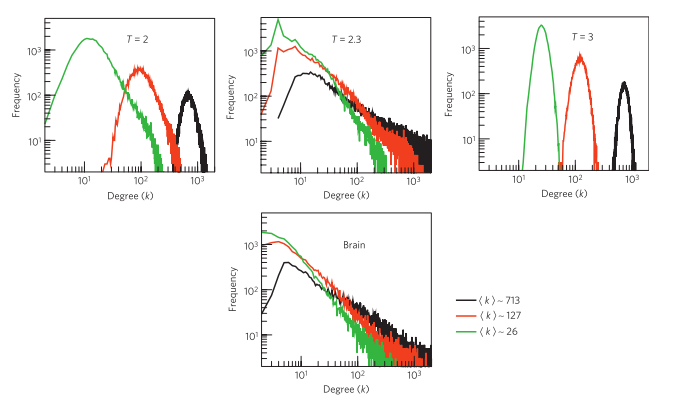
\includegraphics[width=.8\textwidth]{isinglikedynamicschialvo}    
    \caption{\textbf{Ising-like dynamics of the brain.} Degree distributions from fMRI brain data (bottom) and Ising model (top) at temperatures corresponding to subcritical (T=2), critical (T=2.3), and supercritical (3). Black, red, and green curves correspond to average network degrees of 713, 127, and 26, respectively. \cite{Fraiman2009a}}   
   \label{Figure::Ising model and the brain at criticality}   
  \end{center}     
   \end{figure}

\paragraph{Criticisms} The search for qualitative links between empirical data from complex phenomena and simple models should be done cautiously and viewed with some skepticism. The apparent ubiquity of power law relationships in empirical data has been taken by some \cite{Bak1987a} to mean something fundamental, but many others question the validity of this \cite{Stumpf2012a}. In particular, though the rule of thumb for a purported power law says on a log-log plot the relationship should be approximately linear over two orders of magnitude \cite{Sethna2011a}, many published results don't fit this criterion. Rather than following a particular power law, many of these data sets are merely heavy-tailed. However, much of the data concerning neuronal avalanches does span at least two orders of magnitude, or is cut off by the experimental limitation of electrode size. Even if the statistics have been properly dealt with, has anything been gained in borrowing the language of critical phenomena? In the context of criticality in neural systems, the answer is - though not unequivocally - yes. Though ``imbuing them with a vague and mistakenly mystical sense of universality'' \cite{Stumpf2012a} is a mistake, neuronal networks are better understood as a result of the application of the concepts of statistical mechanics and critical phenomena. Though the generative mechanism in the brain is not known (nor within the scope of this paper), there is real functional benefit and thus reason for neuronal networks to operate at criticality: their dynamic range and information capacity is maximized. Thus, though appeals to fundamental insights and underpinnings and notions of universality should be met with some skepticism, there is real functional, biologically and evolutionarily motivated physical insight into the workings of the brain to be found in the study of criticality in neural systems.

\section*{Conclusions}

To conclude, neuronal avalanches following power law relationships in probability distribution of size and duration have been observed and the consequences discussed. Theoretical models and empirical data suggest that these avalanches occur in a critical regime and may be qualitatively and quantitatively understood through the lens of the critical phenomena of statistical physics. In addition, theoretical and experimental results indicate that networks of neurons, and indeed animal and human brains, benefit from maximized dynamic range and information capacity as a result of operating at criticality. Further, qualitative links to statistical physics and in particular the Ising model more firmly establish the role of critical phenomena in neural systems. The significance of these findings is to establish an interdisciplinary field merging complex systems, neuroscience, mathematics, and physics. This emerging field of criticality in neural systems is a promising endeavor which has already yielded great insights into the fundamental workings of the brain. It seems physics may yet have a great deal to contribute to one of the greatest known mysteries: the human brain. 

\bibliographystyle{ieeetr}

\bibliography{Bib}

\end{document}
